\documentclass{article}
\usepackage{graphicx}
\usepackage{listings}
\usepackage{ctex}
\usepackage{graphicx}
\usepackage[a4paper, body={18cm,22cm}]{geometry}
\usepackage{amsmath,amssymb,amstext,wasysym,enumerate,graphicx}
\usepackage{float,abstract,booktabs,indentfirst,amsmath}
\usepackage{array}
\usepackage{booktabs} %调整表格线与上下内容的间隔
\usepackage{multirow}
\usepackage{diagbox}
\usepackage{indentfirst}
\usepackage{bm}
\usepackage{fancyhdr}




\pagestyle{fancy}

\lhead{\bfseries \normalsize 学号:1952033\quad 姓名:侯雅玥 \quad 组员:廖宏 \\实验名称:单管交流放大电路的研究\quad 课程名称:电子技术实验\quad 专业:微电子科学与工程 } 
\rhead{}

\begin{document}

	\section{\zihao{4} 实验名称:单管交流放大电路的研究}
    \section{\zihao{4} 实验目的}
    \zihao {5} (1)通过典型的分压式放大电路的研究,学会检查、调整及测量电路的工作状态	\par
               (2)掌握电路中电压放大倍数、频率响应曲线及通频带的测量方法,学会电压放大倍数理论值的估算方法,研究电路参数变化对放大器性能的影响 \par
    \section{\zihao{4} 实验原理}
    对于阻容耦合共涉及放大器,为使其正常工作而不产生非线性失真,博旭设置合适的静态工作点,静态工作点Q在三极管输入特性线性部分,同时使Q点位于输出特性的放大区,输入型号变化时,工作点始终在放大区内,并要求所设置的静态工作点保持稳定。\par
    \textbf{(1)静态工作点的调整}\par
	如图2,为实验所用的分压式偏置共发射极电路,为使电路正常工作,必须设置合适的静态工作点。其中Ucc,集电极负载Rc,基极电流$I_B$的变化,都会影响静态工作点Q的位置,如图1所示\par
	当基极电流$I_B$减小时,Q沿负载线移动至Q1;当电源电压Ucc变化时,直流负载线左右平移,Q移动至Q2;当集电极负载Rc改变时,直流负载线的斜率发生变化,Q移动至Q3。\par
	当三极管输出特性曲线较为平坦时,Q1点的变化最明显,且改变$I_B$实际上是调节Rw,故通过调节Rw来调节静态工作点。\par
	\begin{figure}[h]
		%\small
		\centering
		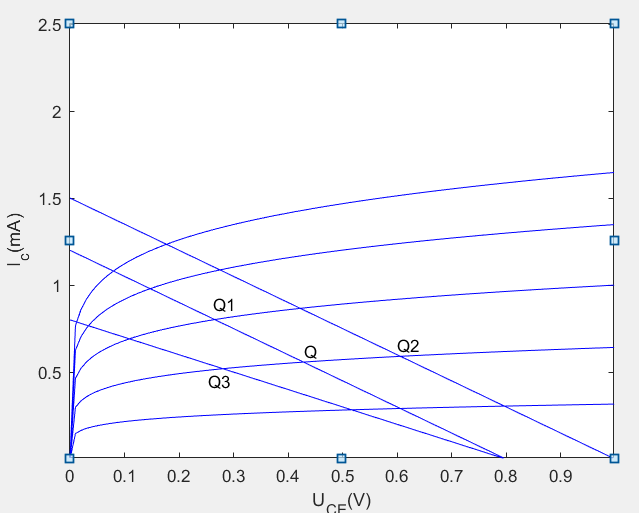
\includegraphics[width=10cm]{H:/电子技术试验/4-4/4-4-2.png}
		\caption{Figure example 1} \label{fig:aa}
	\end{figure}
\newpage
	
	\textbf{(2)放大器增益的测量}\par
	将输入电压Ui加至电路的输入端,当静态工作点合适时,输出信号应当是放大的正弦信号,用$A_u$表示电压的放大倍数,
	\begin{equation*}
		\ A_U=\frac{U_o}{U_i}=-\beta\frac{{R_L}^{'}}{r_{be}},
	\end{equation*}
	\begin{equation*}
		\ {R_L}^{'}=R_c\| R_l,
	\end{equation*}
	\begin{equation*}
		\ r_{be}\approx 200+(1+\beta)\frac{26(mA)}{I_{EQ}(mA)},
	\end{equation*}
	按图2接好电路,使用示波器观察输出不是站的电压波形,同时得到电压Ui和Uo,通过计算得到$A_u$\par

	\textbf{(3)最大不失真输出电压}\par
	$U_omax$是不出现饱和或截止失真时,放大器输出的最大不失真的输出电压,最大不失真电压的峰峰值,即为放大器的输出动态范围,在(1)的基础上,增大输入信号幅度,同时调节Rw观察输出波形,当输出波形出现失真时,$U_o=U_omax$
    	\textbf{(4)放大电路的频率特性}\par
		电压增益在中频增益$A_0$的0。707倍的时候,所对用的频率即为放大器的上线频率$f_H$
		\textbf{(5)负载对放大器增益的影响}\par
         实验中常使用Rc来改变放大倍数
		\section{\zihao{4} 实验电路图}
		\begin{figure}[h]
		%\small
		\centering
		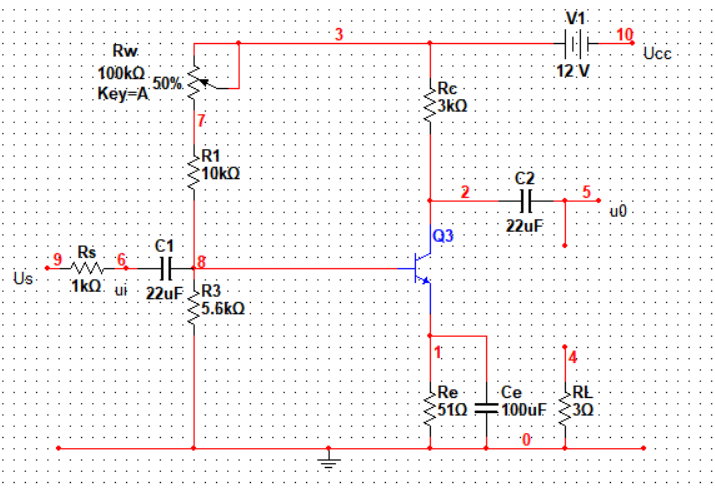
\includegraphics[width=12cm]{H:/电子技术试验/4-4/4-4.png}
		\caption{Figure example 2} \label{fig:aa}
	\end{figure}
\section{\zihao{4} 实验内容及步骤}
\subsection {静态工作点及电压放大倍数的测量}
(1)按照图2连接电路,接通电源,调节Rw使$I_CQ$=2mA  \par
(2)测量$U_{CQ},U_{BQ},U_{EQ}$
(3)分别将$R_w$调至最大和最小,观察截止失真的波形
\subsection{基本放大电路通频带及频幅特性的测量}
(1)$I_CQ$调至2mA,恢复正常静态工作点\par
(2)保持输入信号(5mV)不变,改变输入信号的频率,找到电压降至0.07Uo时对应的信号频率。
\subsection{观察$R_C,R_L$对放大器静态工作点、电压放大倍数的影响}
(1)将Rc改为1k$\omega$\par
(2)测量$U_{CQ},U_{BQ},U_{EQ},U_i,U_0$,计算$A_u$


\begin{table}[h]
	\centering  
	\begin{tabular}{c|c|c|c|c|c|c|c|c}
		\hline
		\multirow{2}{*}{$R_W$} & \multicolumn{4}{c}{工作点测量值} \vline    &  \multirow{2}{*}{$U_i$} & \multirow{2}{*}{$U_0$} & \multicolumn{2}{c}{Au} \\ \cline{2-5} \cline{8-9}	 
		                       & $I_{CQ}$  & $U_{CQ}$ & $U_{BQ}$ & $U_{EQ}$& &                       &实测值                  &理论值\\ \hline
		               正常值   & 2mA     &    6.0V   & 0.696V    &0.50V    &5mV                     &-1.275V                   & -$2.55 \times 10^2$ &  -230 \\   \hline
		                        &  & 1V & & &\multicolumn{4}{c}{(输出波形) $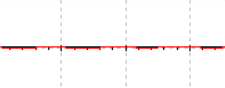
\includegraphics{H:/电子技术试验/4-4/4-44.png}$} \\  \hline
								&  &10V  & & &\multicolumn{4}{c}{(输出波形) $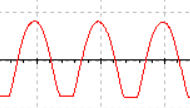
\includegraphics{H:/电子技术试验/4-4/4-43.png}$}\\
		\hline
	\end{tabular}
	\caption{静态工作点及电压放大倍数的测量}\label{SIGN}
	\end{table}

	\begin{table}[h]
		\centering  
		\begin{tabular}{c|c|c|c|c|c|c|c|c|c|c|c|c}
			\hline
			                    $f(Hz)$   & 10     & 20    & 50    & 100   & 200   & 500   & $10^3$ & $5 \times 10^3$ & $10^4$ & $2 \times 10^4$ & $10^5$ & $f_{Hz}$ \\ \hline 
								 Uo(v)    & -0.415  & -0.443 & -0.523 & -0.680 & -0.935 &-1.199  & -1.275  &-1.303            & -1.280  & -1.310           & -1.282  & 185     \\ \hline
			      $A_u=\frac{U_i}{U_0}$   & -83     & -88.6  & -104.6 & -136   & -187   & -239.8 & -255    & -260.6            & -256    & -262            & -256.4  &   \\   \hline
								
			\hline
		\end{tabular}
		\caption{基本放大电路通频带、幅频特性的测量}\label{SIGN}
		\end{table}
\newpage
		\begin{table}[h]
			\centering  
			\begin{tabular}{c|c|c|c|c|c|c|c|c}
				\hline
					      $R_c$    & $R_L$       & $U_{CQ}$ & $U_{BQ}$ & $U_{EQ}$ & $U_i$  & $U_o$  &  $A_u=\frac{U_O}{U_i}$ \\ \hline 
					 $3k\Omega $    & $3k\Omega$  & 6.0V     & 0.696V   & 0.05V    & 0.005V & -1.275V &  -255  \\ \hline
					 $1k\Omega$    & $\infty$    & 2.0V     & 0.696V   & 0.051V   & 0.005V & -0.385V &  -7.7 \\   \hline
									
				\hline
			\end{tabular}
			\caption{观察Rc、RL对放大器静态工作点、电压放大倍数的影响}\label{SIGN}
			\end{table}

	\section{\zihao{4} 实验设备和器材}
	(1)双踪示波器             \qquad \qquad    1台\par
	(2)函数信号发生器          \qquad         1台\par
	(2)直流稳压电源             \qquad \quad  1台\par
	(2)模拟电路实验箱            \qquad  1台\par
	(2)万用表                   \qquad  \qquad \qquad  1只\par
	(2)元器件   
\section{误差处理}

\begin{align*}
	\ u(A_U)=\frac{A_u-A_{u0}}{A_u} \times 100\%=9.8\%
	\end{align*}    \par
(1)误差可能是器件老化造成。\par
(2)三极管存在沟道长度调制效应。

\section{结论}
(1)综上所述,得到静态工作点为$U_{CQ}$为6V时,处于静态工作点。\par
(2)频幅特性如下图3,$f_H$为185Hz\par
(3)Rc和RL会对静态偏置点和放大倍数造成影响。


\section{思考题}
(1)如何调节最佳静态工作点?\par
根据电路器件参数计算得到理论值,然后在测试中调节得到最佳静态工作点\par
(2)电容$C_E$去掉后,静态工作点是否受到影响?电压放大倍数?为什么?\par
静态工作点不受到影响,电压放大倍数不受影响。\par
静态工作点由直流源决定,但是电容器对于直流电路相当于断路,与静态偏置点无关。对于交流电路,电容器相当于短路,因此对于放大倍数没有影响\par
(3)输出端接负载RL后,电压增益是否受到影响\par
由于 $R_L^{'}=R_C\| R_L$ 因此负载RL的值对Au有影响\par
(4)调节放大器的静态工作点Q时,上篇值电阻由RL和Rw组成,能否直接调节Rw?\par
可以直接调节Rw\par
(5)由估算公式$ A_U=\frac{U_o}{U_i}=-\beta\frac{{R_L}^{'}}{r_{be}},$,增大Rc可以提高Au,是否无限增大Rc?为什么?分析有源负载的作用。\par
不可以,Rc的改变会导致静态工作点的改变,要保证放大器在最佳静态工作点。\par
有源负载是一种表现出稳流非线性电阻特性的元件或电路。在电路设计中,有源负载是一种由有源器件组成的电路元件。晶体管等有源器件对小信号产生高阻抗,但不需要很大的直流电压降,这种特性类似于阻值很大的电阻。\par
\begin{figure}[h]
	%\small
	\centering
	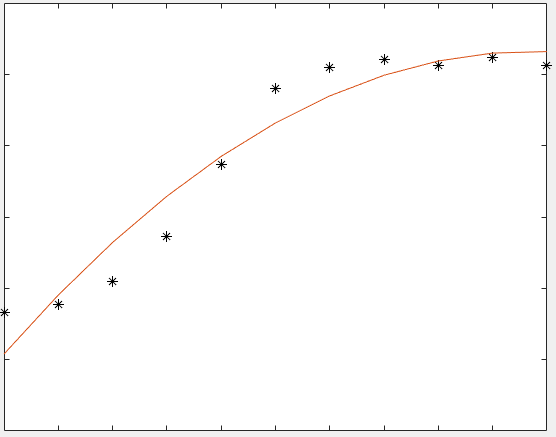
\includegraphics[width=8cm]{H:/电子技术试验/4-4/4-45.png}
	\caption{Figure example 3} \label{fig:aa}
\end{figure}


\end{document}

